\chapter{Proposal: RLCEPS}
\label{ch:proposal}

\section{Program Synthesis in Healthcare}
\label{sec:ps-health}

Automation tools that make use of Machine Learning (also known as Healthcare 4.0 \cite{tortorellaHealthcareTrendsChallenges2020}) have been consistently identified as crucial for reducing the workload of Healthcare professionals and improving the quality of care \cite{agrawalMachineLearningHealthcare2020, deviDesignImplementationAdvanced2022, g.kumarSurveyMachineLearning2016, ganguliMachineLearningPursuit2020, maityMachineLearningImproved2017, mitraMachineLearningHealthcare2021, pianykhImprovingHealthcareOperations2020, xhaferraRoleMachineLearning2022} especially as healthcare systems struggle with understaffing \cite{ashleyy.metcalfHospitalUnitUnderstaffing2016,SurveyShowsHidden1993,UnderstaffingSignificantIssue2012,campbellUniversalHealthCoverage2013, hudsonUnderstaffing2015, mercerMessageEditorinChief2008, r.stanleyUnderstaffedOverwhelmed2010, munnUnderstaffingWardsCompromising2017, thelancetHealthcareSystemStaffing2018}.

Healthcare is also a domain where the advantages of program synthesis (as introduced in section \ref{sec:impacts}) are particularly relevant.
\begin{itemize}
    \item Inadequate \emph{capabilities} of decision systems in Healthcare present particularly challenging risks as patient's health and life can be at stake.
    \item No less dangerous is the risk of perverse incentives and insufficient \emph{alignment} of decision systems with the interests of the patient.
    \item Due to the risks above, Healthcare is a highly regulated domain and \emph{compliance by design} is a crucial feature of any decision systems deployed therein
    \item As a consequence, decision systems in Healthcare are never deployed fully autonomously. Instead, they have to support doctors in making the final decisions and have to be \emph{good team-players}, explaining the rationale behind every suggestion and supporting dialogue.
    \item \emph{Privacy} of clinical data is of utmost importance.
    \item Novel \emph{scientific discoveries} in healthcare have a particularly positive social impact.
\end{itemize}

This makes program synthesis a promising tool for improving the quality of decision systems in Healthcare.

\section{Reinforcement learning in Healthcare}
\label{sec:rl-health}

As discussed in chapter \ref{ch:promise} program synthesis can be applied in imitation learning and reinforcement learning settings.
Imitation learning does not require a complex interplay between learning and collecting experiences and, as a result, is easier and faster.
However, imitation learning has a fundamental limitation: a student can never exceed their master through imitation alone.

We argue that this limitation makes reinforcement learning a necessity for forward-looking healthcare research, and indeed it is gaining traction across a wide variety of healthcare fields \cite{yuReinforcementLearningHealthcare2021}.
Note in particular that program synthesis driven scientific discovery is not possible in a pure imitation learning setting.

Reinforcement learning on live patients is both unethical and infeasible.
Instead, one can take a multi-stage learning approach described on figure \ref{fig:RLCEPS}: 
\begin{enumerate}
  \item Use imitation learning on clinical histories to develop an accurate patient simulator
  \item Use reinforcement learning to develop a decision support system that can potentially achieve better health outcomes for the patient than the clinican
\end{enumerate}

\begin{figure}
  \centering
  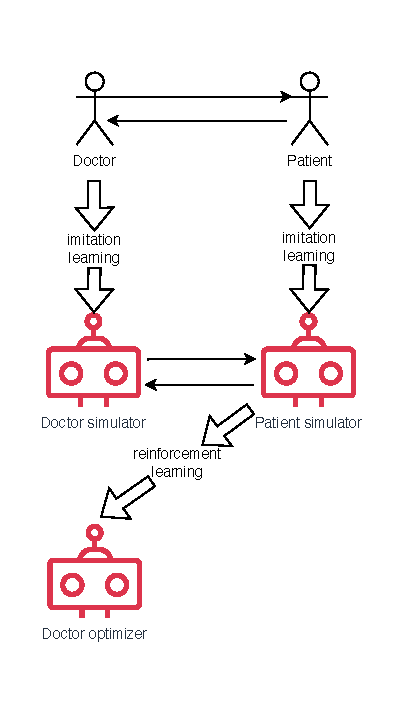
\includegraphics[width=0.9\linewidth]{images/rlceps.pdf}
  \caption{Patient simulator reinforcement learning}
  \label{fig:RLCEPS}
\end{figure}

\newpage
\section{RLCEPS}
\label{sec:patient-sRLCEF}

\begin{highlight}
Reinforcement Learning from Code Evaluation in Patient Simulators (RLCEPS) is \emph{the application of program synthesis methods to solve reinforcement learning environments that simulate patients}.
As the intersection of reinforcement learning and program synthesis in Healthcare, it combines the high degree of expert supervision afforded by program synthesis with the opportunity to exceed human performance in some areas afforded by reinforcement learning.
This makes RLCEPS a powerful framework for developing decision support systems in Healthcare.
\end{highlight}